\documentclass[a4paper,12pt]{article}
\usepackage[margin=1in]{geometry}

\usepackage[T2A]{fontenc}			% кодировка
\usepackage[utf8]{inputenc}			% кодировка исходного текста
\usepackage[english,russian]{babel}	% локализация и переносы
\usepackage{graphicx}                % Математика
\usepackage{amsmath,amsfonts,amssymb,amsthm,mathtools} 
\usepackage{mathtext}
\usepackage[T2A]{fontenc}
\usepackage[utf8]{inputenc}

\usepackage{wasysym}

%Заговолок
\author{Бичина Марина 
группа Б04-005 1 курса ФЭФМ}
\title{}
\date{}


\begin{document} % начало документа

\begin{center}
\begin{Large}
{Бичина Марина Б04-005, Лабораторная работа №. 11.1(1) <<Определение ширины запрещенной зоны полупроводника>>}
\end{Large}
\end{center}
\paragraph{Цель работы:} 
\begin{enumerate}
\itemsep0em
\item Исследовать температурную зависимость проводимости типичного полупроводника 
\item Определить ширину запрещенной зоны 
\end{enumerate}

\paragraph{Теоретическая справка:}
Проводимость в полупроводниках зависит от количества электронов в зоне проводимости и дырок в валентной зоне.

Вероятность заполнения $f(\varepsilon)$ энергетических уровней электронами определяется функцией Ферми:
$$
f(\varepsilon) = \frac{1}{1+\exp\left(\frac{\varepsilon - \mu}{kT}\right)},
$$
где $\varepsilon$ -- значение энергии уровня в зоне проводимости, $\mu$ -- уровень Ферми. В приближении $(\varepsilon-\mu)>>kT$ имеем:

$$
f(\varepsilon) \approx \exp \left( - \frac{\varepsilon - \mu}{kT} \right).
$$

При небольших температурах электроны занимают нижние уровни, то есть $\varepsilon \approx \varepsilon_{c}$, 
$\varepsilon_{c}$ -- энергия, соответствующая дну зоны проводимости. Тогда количество электронов $n_n$
равно:
$$
n_{n}=Q_{n} \cdot f(\varepsilon) \approx Q_{n} \exp \left(-\frac{\varepsilon_{c}-\mu}{k T}\right).
$$
Здесь $Q_n$ -- количество занятых электронами уровней.
Вероятность возникновения дырки равна $1 - f(\varepsilon).$ В рассматриваемом приближении энергию дырок будем считать равной энергии верхней границы валентной зоны $\varepsilon$, тогда число дырок $n_p$ в валентной зоне определяется аналогично
$$
n_{p}=Q_{p} \cdot (1-f(\varepsilon)) \approx Q_{p} \exp \left(\frac{\varepsilon_{v}-\mu}{k T}\right).
$$
В чистых полупроводниках $n_n \approx n_p$, следовательно верно:
$$
n_{n} n_{p}=n^{2}=Q_{n} Q_{p} \exp \left(-\frac{\varepsilon_{c}-\varepsilon_{v}}{k T}\right).
$$
Ширину запрещенной зоны обозначим $\Delta=\varepsilon_{c}-\varepsilon_{v}$, тогда получим:
$$
n \propto \exp \left(-\frac{\Delta}{2 k T}\right).
$$
В присутствии электрического поля $Е$ средняя скорость $v$ носителя заряда
пропорциональна eмy: $v \propto E$.
Плотность тока в случае полупроводника запишется так: $$ j=j_n+j_p=|e|\left(n_n v_n+n_p v_p\right) \propto nE, $$ где
индексы $n$ и $p$ соответствуют электронам и дьркам. Из полученной пропорциональности
следует температурная зависимость проводимости полупроводника:
\begin{equation}
\sigma_{s} \propto \exp \left(-\frac{\Delta}{2 k T}\right)
\label{s}
\end{equation}
\newpage

\paragraph{Описание установки:}
\paragraph{}
В нашей работе производится исследование зависимости $\sigma(T)$ с помощью универсального цифрового вольтметра В7-34А
\begin{figure}[h!]
\centering
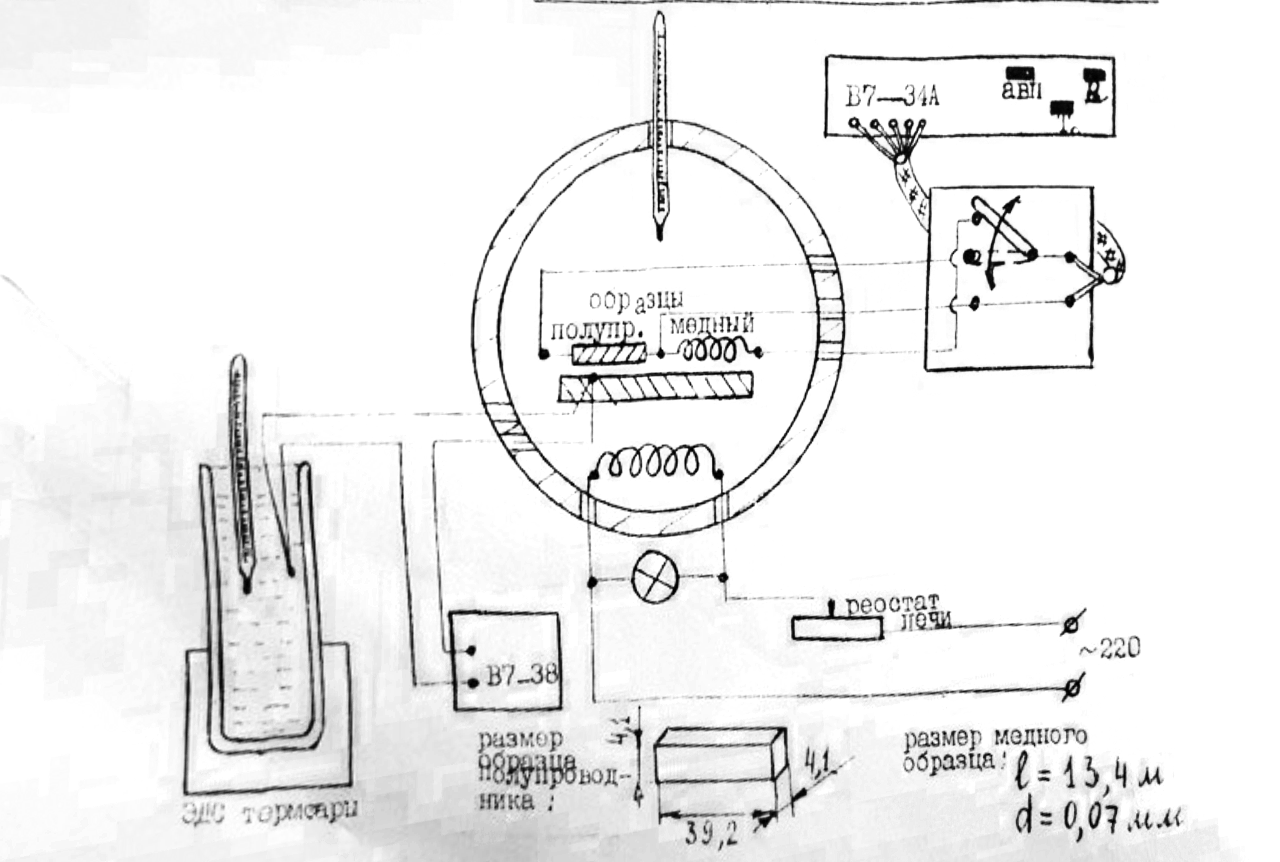
\includegraphics[scale=0.4]{setup_1.png} 
\caption{Схема установки по измерению $\sigma(T)$}
\end{figure}

Исследуемые образцы в специальном зажиме помещаются в электронагревательную печь. Сопротивление образцов измеряется с помощью вольтметра B7-34A. Поочередное подключение образцов к прибору осуществляется с помощью ключа.\\
Удельная проводимость образцов находится по формуле 
\begin{equation}
\sigma = \frac{l}{RS}
\label{sigma}
\end{equation}
где R -- сопротивление образца, l -- его длина, S -- поперечное сечение образца.\\
Константы при выполнении работы: 
\begin{enumerate}
\itemsep0em
\item Константа термопары: $0.41\; \dfrac{\text{мВ}}{^oC}$
\item Истинный 0: $T_t = -0.01$ мВ
\item Температура в помещении $T_k = 25 ^oC$
\item Размер медного образца $l = 13.4 \;\text{м}, \;d = 0.07\;\text{мм}$
\item Размер полупроводника: $ c=39.2 \;\text{мм}, \; a=b= 4.1\;\text{мм} $
\end{enumerate}
\paragraph{Ход работы:}
\begin{enumerate}
\itemsep0em
\item В ходе нагревания образцов, снимем температурную зависимость R(T). По формуле \ref{sigma} найдем значение удельной проводимости образцов. Результаты занесем в таблицу 1 
\begin{table}[h!]
\centering
\begin{tabular}{|l|l|l|l|l|l|}
\hline
$\Delta$T, мВ & R\_1, кОм & R\_2, кОм & $\Delta$T, K & $\sigma_1$, Oм*м $^{-1}$ & $\sigma_2$, Ом*м$^{-1}$ \\ \hline
0,02          & 0,0914   & -        & 0,49         & 9524133,15               &                         \\ \hline
0,13          & 0,0924   & 0,5957   & 3,17         & 9421058,12               & 3,91                    \\ \hline
0,32          & 0,094    & 0,4572   & 7,80         & 9260699,68               & 5,10                    \\ \hline
0,72          & 0,0972   & 0,2913   & 17,56        & 8955820,68               & 8,01                    \\ \hline
1,03          & 0,0997   & 0,2136   & 25,12        & 8731251,46               & 10,92                   \\ \hline
1,32          & 0,102    & 0,16     & 32,20        & 8534370,30               & 14,57                   \\ \hline
1,52          & 0,1036   & 0,1344   & 37,07        & 8402565,35               & 17,35                   \\ \hline
1,72          & 0,1053   & 0,113    & 41,95        & 8266911,40               & 20,64                   \\ \hline
1,94          & 0,107    & 0,094    & 47,32        & 8135567,95               & 24,81                   \\ \hline
2,15          & 0,1086   & 0,0812   & 52,44        & 8015706,91               & 28,72                   \\ \hline
2,33          & 0,1104   & 0,0707   & 56,83        & 7885016,04               & 32,98                   \\ \hline
2,52          & 0,1116   & 0,0616   & 61,46        & 7800230,92               & 37,86                   \\ \hline
2,76          & 0,1134   & 0,0522   & 67,32        & 7676417,73               & 44,67                   \\ \hline
2,95          & 0,1153   & 0,0577   & 71,95        & 7549919,95               & 40,41                   \\ \hline
3,16          & 0,1165   & 0,0438   & 77,07        & 7472152,54               & 53,24                   \\ \hline
3,25          & 0,1173   & 0,0385   & 79,27        & 7421191,56               & 60,57                   \\ \hline
3,4           & 0,1183   & 0,0352   & 82,93        & 7358459,60               & 66,25                   \\ \hline
\end{tabular}
\caption{Данные, полученные в ходе выполнения работы}
\end{table}
\item По полученным данным построим график зависимости $\sigma(T)$ для меди
\begin{figure}[h!]
\centering
\includegraphics[scale=0.75]{../../../../Users/Marina/Documents/labs/plot_Cu.png} 
\end{figure}
\item Определим температурный коэффициент сопротивления для меди. Для этого угловой коэффициент поделим на среднее значение $\sigma$:
\begin{equation*}
\alpha = \frac{a}{\sigma} = 0.00268\; K^{-1}
\end{equation*}
Погрешность для температурного коэффициента возьмем из погрешности для углового коэффициента. \\ Окончательно:
\[\alpha = (2.70 \pm 0.05)\cdot 10^{-3} \; K^{-1}\]
\item Получим графики для полупроводника (с экспоненциальной и линейной зависимостями)
\begin{figure}[h!]
\centering
\includegraphics[scale=0.75]{../../../../Users/Marina/Documents/labs/plot_exp.png} 
\end{figure}
\begin{figure}[h!]
\centering
\includegraphics[scale=0.75]{../../../../Users/Marina/Documents/labs/plot_Si.png} 
\end{figure}
\item По наклону графика 3 определим, исходя из формулы \ref{s}, ширину запрещенной зоны, как
\[		\Delta = 2k \frac{\Delta(\ln \sigma)}{\Delta (1/T)}  = -2k\cdot a\]

где а -- угловой коэффициент, вычисленный по МНК
\[\Delta = 2\cdot 1.38\cdot 10^{-23}\cdot 4\cdot 10^3 = 11.04 \cdot 10^{-20}\text{Дж} = 0.689\; \text{эВ}\]
Данное значение соответствует запрещенной зоне Германия 
\item Значение погрешности вычислим как \[\sigma_{\Delta} = \frac{2k}{e}\cdot \sigma_a = 1 \cdot 10^{-4} эВ\] 
Окончательно:
\[\Delta = 0.6890\pm0.0001 \;\text{эВ}\]
\end{enumerate}
\paragraph{Выводы:}
\begin{enumerate}
\item В ходе работы была исследована температурная зависимость проводимости меди и германия. Получено, что для меди зависимость выглядит как $\sigma \propto 1/T$, а для германия как $\sigma \propto exp(-1/T)$
\item Был вычислен температурный коэффициент сопротивления меди, равный \[\alpha = (2.70\pm 0.05)\cdot 10^{-3}\;\;K^{-1}\]
при табличном значении 
\[\alpha_{\text{табл}} = 3.8 \cdot 10^{-3}\;\;K^{-1}\]
\item Была вычислена ширина запрещенной зоны полупроводника
\[\Delta = 0.6890\pm0.0001 \;\text{эВ}\]
с хорошей точностью совпадающая с запрещенной зоной Германия 
\[\Delta_{\text{табл}} = 0.67 \;\text{эВ}\]
\end{enumerate}
\end{document}